\subsection{Theory Exercises}

\subsubsection*{Bishop 11.3}

To transform a random variable \( z \sim \text{Uniform}(0, 1) \) into a random variable \( y \) with the Cauchy distribution 
\[
p(y) = \frac{1}{\pi} \frac{1}{1 + y^2},
\]
We Firstly determine the CDF of the Cauchy distribution
\[
F_Y(y) = \int_{-\infty}^y \frac{1}{\pi} \frac{1}{1 + t^2} \, dt = \frac{1}{\pi} \arctan(y) + \frac{1}{2}.
\]
To map \( z \sim \text{Uniform}(0, 1) \) to \( y \sim p(y) \), we set:
\[
F_Y(y) = z.
\]
And solve for y
\[
\frac{1}{\pi} \arctan(y) + \frac{1}{2} = z.
\]
\[
\arctan(y) = \pi z - \frac{\pi}{2}.
\]
Taking the tangent of both sides:
\[
y = \tan\left(\pi z - \frac{\pi}{2}\right).
\]
We can conclude that the transformation is given by:
\[
y = \tan\left(\pi z - \frac{\pi}{2}\right) \quad \text{or equivalently} \quad y = -\cot(\pi z).
\]


\subsection{Programming Exercise}
The code is shown in~\cref{sec:week3:code:exercise}.
\begin{enumerate}
  \item We used proposal distribution $unif([-3,3])$ with $k=24$
  \item We used proposal distribution $\mathcal{N}(0,1) $ with $k=10$ \\
   The plot below shows that the two scaled proposal distributions provide an upper bound on the unnormalized target distribution.
  \begin{center}
      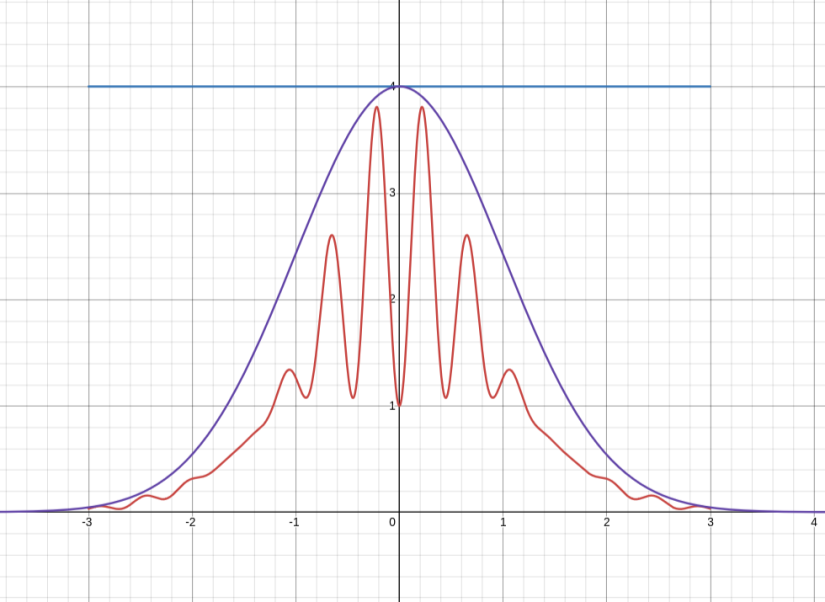
\includegraphics[width=10cm]{./figures/proposals.png}
  \end{center}
  \item This uses the proposal $\mathcal{N}(0,1)$ to firstly approximate the importance distribution (We used 1000 proposal samples), then samples are drawn from this new distribution.
  \item Comparison plot (1000 experiments)
  \begin{center}
      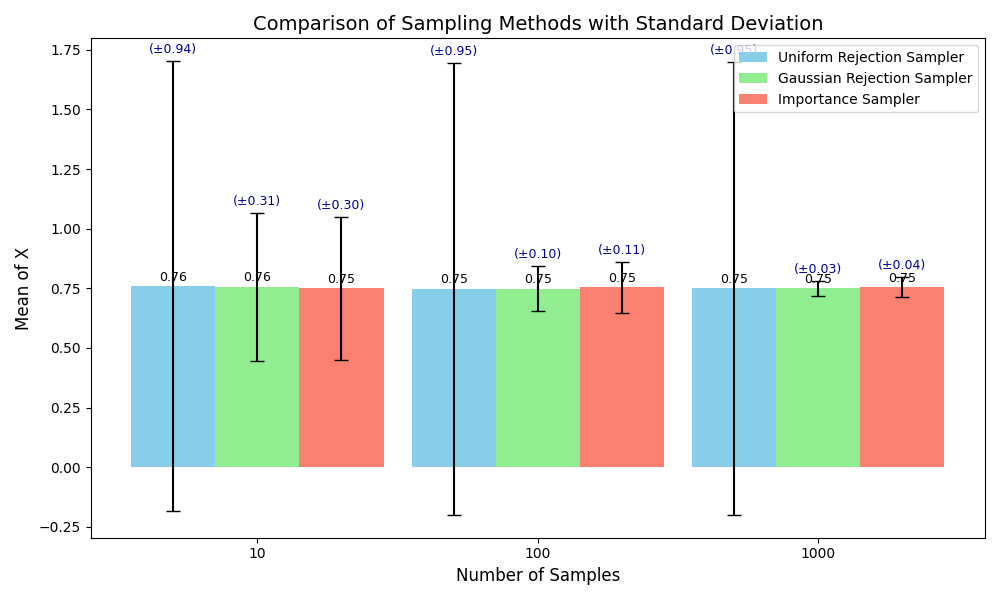
\includegraphics[width=12cm]{./figures/comparison1.png}
  \end{center}
  From this comparison we can notice that all of the methods produce unbiased results.
  The uniform rejection sampler has the highest variance in general, 
  and we can also notice that it doesn't change with the number of samples.
  The Gaussian rejection and importance sampler seem the same performance overall,
  with variance that scaled nicely with the number of samples
  (theoretically the importance sampler should be slightly worse).
\end{enumerate}


\subsection{Pyro}

The code is shown in~\cref{sec:week3:code:pyro}.
The plot of the GMM samples is shown in~\cref{fig:week3:pyro:gmm-samples}.
The plots of the densities $p(x_2 | x_1 = 2)$ and $p(x_2 | x_1 = 3)$
are shown in~\cref{fig:week3:pyro:cond-pdf}.

\begin{figure}[htbp]
  \centering
  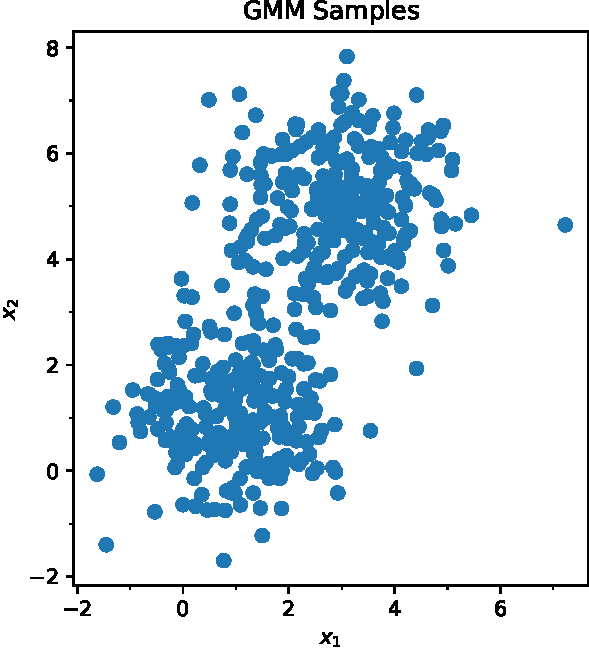
\includegraphics[width=0.5\textwidth]{./figures/gmm_samples.pdf}
  \caption{Scatter plot of 500 samples of the GMM.}
  \label{fig:week3:pyro:gmm-samples}
\end{figure}

\begin{figure}[htbp]
  \centering
  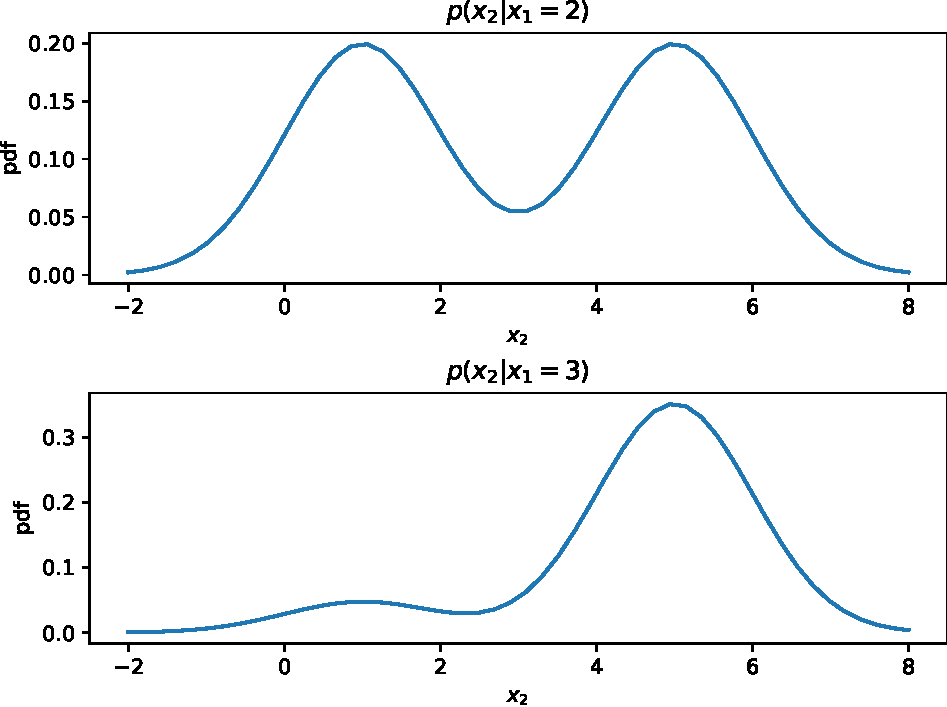
\includegraphics[width=0.7\textwidth]{./figures/cond_pdf.pdf}
  \caption{
    PDF of conditionals on $x_1$ of the GMM.
  }
  \label{fig:week3:pyro:cond-pdf}
\end{figure}
